\documentclass[10pt]{beamer}
\usepackage[utf8]{inputenc}
\usepackage{tikz, pgfplots}
\pgfplotsset{compat=1.18}
\usetikzlibrary{positioning}
\usetikzlibrary{trees}
\usetikzlibrary{shapes.geometric, arrows.meta, positioning}
\usepackage{xcolor}
\usetheme{EastLansing}
\usepackage{graphicx}
\usepackage{subcaption}
\usepackage{hyperref} 
\usepackage{colortbl} % Required for \rowcolor
\usepackage{animate}
\usepackage[T1]{fontenc}
\usepackage{amsmath, amsfonts, amssymb}
\usepackage[french]{babel}
\setbeamertemplate{caption}[numbered]

\title{Rapport Hebdo}
\author{Viet Anh Quach}
\institute{3SR}
\date{\today}

\begin{document}

\begin{frame}
    \titlepage
\end{frame}


\section{MPM}



\section{DEM}
\begin{frame}{Étude sur le critère de rupture de Coulomb}
    \begin{table}
        \centering
        \begin{tabular}{|c|c|c|c|}
            \hline
            \textbf{Symboles}               & \textbf{Paramètres}         & \textbf{Valeurs}                          & \textbf{Unité}  \\
            \hline
            Nombre de particules            & N                           & $15^3$                                    & -               \\
            \hline
            Le rayon des particules         & R                           & 0.003 $\div$ 0.005                        & m               \\
            \hline
            Masse volumique                 & $\rho$                      & 2500                                      & $\text{kg/m}^3$ \\
            \hline
            Contrainte isotrope             & $\sigma_{xx} = \sigma_{zz}$ & 100, 200, 300                             & kPa             \\
            \hline
            Raideur normale et tangentielle & $k_n$ \& $k_t$              & \textcolor{black}{$3 \times 10^6$}        & $\text{N/m}$    \\
            \hline
            Niveau de raideur               & $\kappa$                    & 1000                                      & -               \\
            \hline
            Coefficient de frottement       & $\mu$                       & 0.5                                       & -               \\
            \hline
            Déformation axiale              & $\varepsilon_{\text{yy}}$   & 10                                        & $\%$            \\
            \hline
            Masse de la cellule périodique  & $h_{mass}$                  & \textcolor{black}{$7.13 \times 10^{-4}$}  & $\text{kg}$     \\
            \hline
            Nombre d’inertie                & I                           & \textcolor{red}{$10^{-6}\  \& \ 10^{-2}$} & -               \\
            \hline
            Vitesse imposée                 & v                           & $10^{-3}\  \& \ 10 $                      & m/s             \\
            \hline
            Pas de temps                    & $d_t$                       & $10^{-6}\  \& \ 10^{-10}$                 & $\text{s}$      \\
            \hline
            Coefficient d'amortissement     & $\alpha$                    & \textcolor{black}{$0.0 \ \& \ 0.7$}       & -               \\
            \hline
        \end{tabular}
        \caption{Valeurs des paramètres utilisés dans la compression triaxiale}
    \end{table}
\end{frame}




\begin{frame}{Déformation des échantillons lâches}
    \begin{columns}
        \begin{column}{0.5\textwidth}
            \begin{figure}[h]
                \centering
                \animategraphics[loop,autoplay,width=4cm]{10}{Statique_LACHE_}{1}{5}
                \caption{Statique}
            \end{figure}
        \end{column}
        \begin{column}{0.5\textwidth}
            \begin{figure}[h]
                \centering
                \animategraphics[loop,autoplay,width=4cm]{10}{Dynamique_LACHE_}{1}{5}
                \caption{Dynamique}
            \end{figure}
        \end{column}
    \end{columns}
    La vitesse de compression trop élevée, les grains n'ont pas le temps de se réarranger. \\
    Pendant ce temps, les liaisons sont déjà rompues; \\
    $\rightarrow$ La rupture précoce similaire à celle observée pour les échantillons denses.
\end{frame}


\begin{frame}{L'étude sur l'effet dynamique}
    \begin{columns}
        \begin{column}{0.5\textwidth}
            \begin{figure}[h]
                \centering
                \scalebox{0.5}{% GNUPLOT: LaTeX picture with Postscript
\begingroup
  \makeatletter
  \providecommand\color[2][]{%
    \GenericError{(gnuplot) \space\space\space\@spaces}{%
      Package color not loaded in conjunction with
      terminal option `colourtext'%
    }{See the gnuplot documentation for explanation.%
    }{Either use 'blacktext' in gnuplot or load the package
      color.sty in LaTeX.}%
    \renewcommand\color[2][]{}%
  }%
  \providecommand\includegraphics[2][]{%
    \GenericError{(gnuplot) \space\space\space\@spaces}{%
      Package graphicx or graphics not loaded%
    }{See the gnuplot documentation for explanation.%
    }{The gnuplot epslatex terminal needs graphicx.sty or graphics.sty.}%
    \renewcommand\includegraphics[2][]{}%
  }%
  \providecommand\rotatebox[2]{#2}%
  \@ifundefined{ifGPcolor}{%
    \newif\ifGPcolor
    \GPcolortrue
  }{}%
  \@ifundefined{ifGPblacktext}{%
    \newif\ifGPblacktext
    \GPblacktextfalse
  }{}%
  % define a \g@addto@macro without @ in the name:
  \let\gplgaddtomacro\g@addto@macro
  % define empty templates for all commands taking text:
  \gdef\gplbacktext{}%
  \gdef\gplfronttext{}%
  \makeatother
  \ifGPblacktext
    % no textcolor at all
    \def\colorrgb#1{}%
    \def\colorgray#1{}%
  \else
    % gray or color?
    \ifGPcolor
      \def\colorrgb#1{\color[rgb]{#1}}%
      \def\colorgray#1{\color[gray]{#1}}%
      \expandafter\def\csname LTw\endcsname{\color{white}}%
      \expandafter\def\csname LTb\endcsname{\color{black}}%
      \expandafter\def\csname LTa\endcsname{\color{black}}%
      \expandafter\def\csname LT0\endcsname{\color[rgb]{1,0,0}}%
      \expandafter\def\csname LT1\endcsname{\color[rgb]{0,1,0}}%
      \expandafter\def\csname LT2\endcsname{\color[rgb]{0,0,1}}%
      \expandafter\def\csname LT3\endcsname{\color[rgb]{1,0,1}}%
      \expandafter\def\csname LT4\endcsname{\color[rgb]{0,1,1}}%
      \expandafter\def\csname LT5\endcsname{\color[rgb]{1,1,0}}%
      \expandafter\def\csname LT6\endcsname{\color[rgb]{0,0,0}}%
      \expandafter\def\csname LT7\endcsname{\color[rgb]{1,0.3,0}}%
      \expandafter\def\csname LT8\endcsname{\color[rgb]{0.5,0.5,0.5}}%
    \else
      % gray
      \def\colorrgb#1{\color{black}}%
      \def\colorgray#1{\color[gray]{#1}}%
      \expandafter\def\csname LTw\endcsname{\color{white}}%
      \expandafter\def\csname LTb\endcsname{\color{black}}%
      \expandafter\def\csname LTa\endcsname{\color{black}}%
      \expandafter\def\csname LT0\endcsname{\color{black}}%
      \expandafter\def\csname LT1\endcsname{\color{black}}%
      \expandafter\def\csname LT2\endcsname{\color{black}}%
      \expandafter\def\csname LT3\endcsname{\color{black}}%
      \expandafter\def\csname LT4\endcsname{\color{black}}%
      \expandafter\def\csname LT5\endcsname{\color{black}}%
      \expandafter\def\csname LT6\endcsname{\color{black}}%
      \expandafter\def\csname LT7\endcsname{\color{black}}%
      \expandafter\def\csname LT8\endcsname{\color{black}}%
    \fi
  \fi
    \setlength{\unitlength}{0.0500bp}%
    \ifx\gptboxheight\undefined%
      \newlength{\gptboxheight}%
      \newlength{\gptboxwidth}%
      \newsavebox{\gptboxtext}%
    \fi%
    \setlength{\fboxrule}{0.5pt}%
    \setlength{\fboxsep}{1pt}%
    \definecolor{tbcol}{rgb}{1,1,1}%
\begin{picture}(7200.00,5040.00)%
    \gplgaddtomacro\gplbacktext{%
      \csname LTb\endcsname%%
      \put(946,704){\makebox(0,0)[r]{\strut{}$0$}}%
      \csname LTb\endcsname%%
      \put(946,1390){\makebox(0,0)[r]{\strut{}$200$}}%
      \csname LTb\endcsname%%
      \put(946,2076){\makebox(0,0)[r]{\strut{}$400$}}%
      \csname LTb\endcsname%%
      \put(946,2762){\makebox(0,0)[r]{\strut{}$600$}}%
      \csname LTb\endcsname%%
      \put(946,3447){\makebox(0,0)[r]{\strut{}$800$}}%
      \csname LTb\endcsname%%
      \put(946,4133){\makebox(0,0)[r]{\strut{}$1000$}}%
      \csname LTb\endcsname%%
      \put(946,4819){\makebox(0,0)[r]{\strut{}$1200$}}%
      \csname LTb\endcsname%%
      \put(1078,484){\makebox(0,0){\strut{}$0$}}%
      \csname LTb\endcsname%%
      \put(2223,484){\makebox(0,0){\strut{}$2$}}%
      \csname LTb\endcsname%%
      \put(3368,484){\makebox(0,0){\strut{}$4$}}%
      \csname LTb\endcsname%%
      \put(4513,484){\makebox(0,0){\strut{}$6$}}%
      \csname LTb\endcsname%%
      \put(5658,484){\makebox(0,0){\strut{}$8$}}%
      \csname LTb\endcsname%%
      \put(6803,484){\makebox(0,0){\strut{}$10$}}%
    }%
    \gplgaddtomacro\gplfronttext{%
      \csname LTb\endcsname%%
      \put(341,2761){\rotatebox{-270}{\makebox(0,0){\strut{}$q$ (kPa)}}}%
      \put(3940,154){\makebox(0,0){\strut{}$\varepsilon_{yy}$ (\%)}}%
      \csname LTb\endcsname%%
      \put(6104,4602){\makebox(0,0)[r]{\strut{}sD300}}%
      \csname LTb\endcsname%%
      \put(6104,4462){\makebox(0,0)[r]{\strut{}sL300}}%
      \csname LTb\endcsname%%
      \put(6104,4322){\makebox(0,0)[r]{\strut{}sD300}}%
      \csname LTb\endcsname%%
      \put(6104,4182){\makebox(0,0)[r]{\strut{}sL300}}%
    }%
    \gplbacktext
    \put(0,0){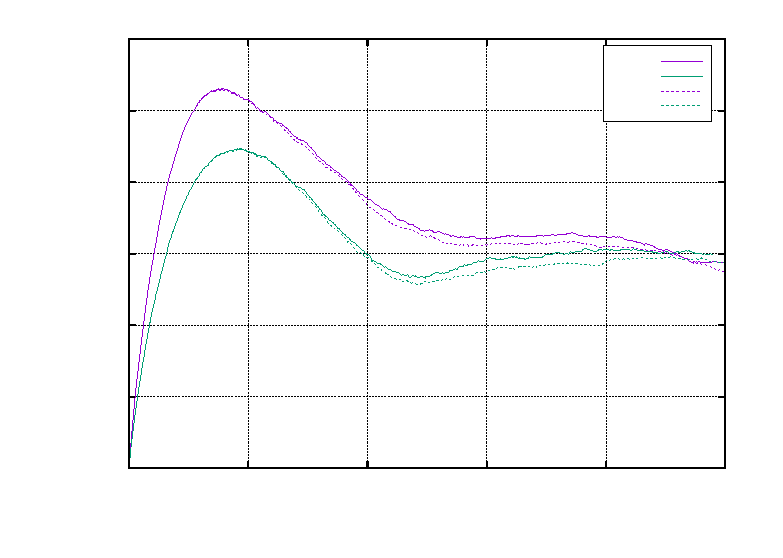
\includegraphics[width={360.00bp},height={252.00bp}]{./dVerlet_Contrainte_Deformation}}%
    \gplfronttext
  \end{picture}%
\endgroup
}
                \caption{Courbe Contrainte-Déformation}
            \end{figure}
        \end{column}


        \begin{column}{0.5\textwidth}
            \begin{figure}[h]
                \centering
                \scalebox{0.5}{% GNUPLOT: LaTeX picture with Postscript
\begingroup
  \makeatletter
  \providecommand\color[2][]{%
    \GenericError{(gnuplot) \space\space\space\@spaces}{%
      Package color not loaded in conjunction with
      terminal option `colourtext'%
    }{See the gnuplot documentation for explanation.%
    }{Either use 'blacktext' in gnuplot or load the package
      color.sty in LaTeX.}%
    \renewcommand\color[2][]{}%
  }%
  \providecommand\includegraphics[2][]{%
    \GenericError{(gnuplot) \space\space\space\@spaces}{%
      Package graphicx or graphics not loaded%
    }{See the gnuplot documentation for explanation.%
    }{The gnuplot epslatex terminal needs graphicx.sty or graphics.sty.}%
    \renewcommand\includegraphics[2][]{}%
  }%
  \providecommand\rotatebox[2]{#2}%
  \@ifundefined{ifGPcolor}{%
    \newif\ifGPcolor
    \GPcolortrue
  }{}%
  \@ifundefined{ifGPblacktext}{%
    \newif\ifGPblacktext
    \GPblacktextfalse
  }{}%
  % define a \g@addto@macro without @ in the name:
  \let\gplgaddtomacro\g@addto@macro
  % define empty templates for all commands taking text:
  \gdef\gplbacktext{}%
  \gdef\gplfronttext{}%
  \makeatother
  \ifGPblacktext
    % no textcolor at all
    \def\colorrgb#1{}%
    \def\colorgray#1{}%
  \else
    % gray or color?
    \ifGPcolor
      \def\colorrgb#1{\color[rgb]{#1}}%
      \def\colorgray#1{\color[gray]{#1}}%
      \expandafter\def\csname LTw\endcsname{\color{white}}%
      \expandafter\def\csname LTb\endcsname{\color{black}}%
      \expandafter\def\csname LTa\endcsname{\color{black}}%
      \expandafter\def\csname LT0\endcsname{\color[rgb]{1,0,0}}%
      \expandafter\def\csname LT1\endcsname{\color[rgb]{0,1,0}}%
      \expandafter\def\csname LT2\endcsname{\color[rgb]{0,0,1}}%
      \expandafter\def\csname LT3\endcsname{\color[rgb]{1,0,1}}%
      \expandafter\def\csname LT4\endcsname{\color[rgb]{0,1,1}}%
      \expandafter\def\csname LT5\endcsname{\color[rgb]{1,1,0}}%
      \expandafter\def\csname LT6\endcsname{\color[rgb]{0,0,0}}%
      \expandafter\def\csname LT7\endcsname{\color[rgb]{1,0.3,0}}%
      \expandafter\def\csname LT8\endcsname{\color[rgb]{0.5,0.5,0.5}}%
    \else
      % gray
      \def\colorrgb#1{\color{black}}%
      \def\colorgray#1{\color[gray]{#1}}%
      \expandafter\def\csname LTw\endcsname{\color{white}}%
      \expandafter\def\csname LTb\endcsname{\color{black}}%
      \expandafter\def\csname LTa\endcsname{\color{black}}%
      \expandafter\def\csname LT0\endcsname{\color{black}}%
      \expandafter\def\csname LT1\endcsname{\color{black}}%
      \expandafter\def\csname LT2\endcsname{\color{black}}%
      \expandafter\def\csname LT3\endcsname{\color{black}}%
      \expandafter\def\csname LT4\endcsname{\color{black}}%
      \expandafter\def\csname LT5\endcsname{\color{black}}%
      \expandafter\def\csname LT6\endcsname{\color{black}}%
      \expandafter\def\csname LT7\endcsname{\color{black}}%
      \expandafter\def\csname LT8\endcsname{\color{black}}%
    \fi
  \fi
    \setlength{\unitlength}{0.0500bp}%
    \ifx\gptboxheight\undefined%
      \newlength{\gptboxheight}%
      \newlength{\gptboxwidth}%
      \newsavebox{\gptboxtext}%
    \fi%
    \setlength{\fboxrule}{0.5pt}%
    \setlength{\fboxsep}{1pt}%
    \definecolor{tbcol}{rgb}{1,1,1}%
\begin{picture}(7200.00,5040.00)%
    \gplgaddtomacro\gplbacktext{%
      \csname LTb\endcsname%%
      \put(682,704){\makebox(0,0)[r]{\strut{}$-1$}}%
      \csname LTb\endcsname%%
      \put(682,1292){\makebox(0,0)[r]{\strut{}$0$}}%
      \csname LTb\endcsname%%
      \put(682,1880){\makebox(0,0)[r]{\strut{}$1$}}%
      \csname LTb\endcsname%%
      \put(682,2468){\makebox(0,0)[r]{\strut{}$2$}}%
      \csname LTb\endcsname%%
      \put(682,3055){\makebox(0,0)[r]{\strut{}$3$}}%
      \csname LTb\endcsname%%
      \put(682,3643){\makebox(0,0)[r]{\strut{}$4$}}%
      \csname LTb\endcsname%%
      \put(682,4231){\makebox(0,0)[r]{\strut{}$5$}}%
      \csname LTb\endcsname%%
      \put(682,4819){\makebox(0,0)[r]{\strut{}$6$}}%
      \csname LTb\endcsname%%
      \put(814,484){\makebox(0,0){\strut{}$0$}}%
      \csname LTb\endcsname%%
      \put(2012,484){\makebox(0,0){\strut{}$2$}}%
      \csname LTb\endcsname%%
      \put(3210,484){\makebox(0,0){\strut{}$4$}}%
      \csname LTb\endcsname%%
      \put(4407,484){\makebox(0,0){\strut{}$6$}}%
      \csname LTb\endcsname%%
      \put(5605,484){\makebox(0,0){\strut{}$8$}}%
      \csname LTb\endcsname%%
      \put(6803,484){\makebox(0,0){\strut{}$10$}}%
    }%
    \gplgaddtomacro\gplfronttext{%
      \csname LTb\endcsname%%
      \put(209,2761){\rotatebox{90}{\makebox(0,0){\strut{}$\varepsilon_{v}$ (\%)}}}%
      \put(3808,154){\makebox(0,0){\strut{}$\varepsilon_{yy}$ (\%)}}%
      \csname LTb\endcsname%%
      \put(1450,4606){\makebox(0,0)[r]{\strut{}dD300}}%
      \csname LTb\endcsname%%
      \put(1450,4456){\makebox(0,0)[r]{\strut{}dL300}}%
      \csname LTb\endcsname%%
      \put(1450,4306){\makebox(0,0)[r]{\strut{}dD300}}%
      \csname LTb\endcsname%%
      \put(1450,4156){\makebox(0,0)[r]{\strut{}dL300}}%
    }%
    \gplbacktext
    \put(0,0){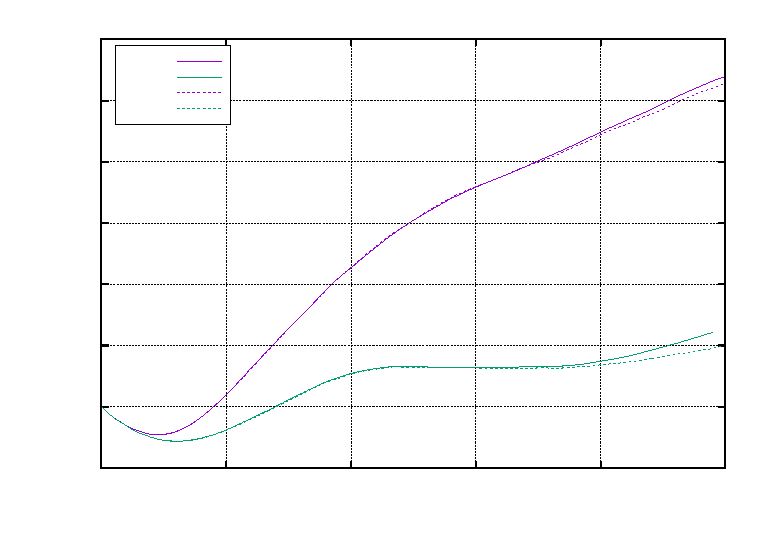
\includegraphics[width={360.00bp},height={252.00bp}]{./dVerlet_Deformation_Volumique}}%
    \gplfronttext
  \end{picture}%
\endgroup
}
                \caption{Déformation Volumique}
            \end{figure}
        \end{column}
    \end{columns}
    \begin{itemize}
        \item Les échantillons lâches se comportent dans une tendence comme l'échantillons denses sous l'effet dynamique.
        \item Le sable lâche n'est pas purement contractant sous compression dynamique.
        \item Néanmoins, l’état critique est toujours observé, même dans le cas dynamique.
    \end{itemize}
\end{frame}







\end{document}
